\clearpage
\chapter{Mastery Workbook 8}

% Chapter page
\section{Induction Mastery Workbook}

\horizontalline{0}{0}

\begin{center}
    \Large{\textbf{I have neither given nor received unauthorized assistance.}}
    \horizontalline{0}{0}
    \large{\textbf{Taylor James Larrechea}}
    \horizontalline{0}{0}
\end{center}

% Problem 1
\begin{problem}{Problem 1}
    \begin{statement}{Problem Statement}
        With paper and pencil (or online tablet but not typing), add the numbers 1 - 100 any way you like. Do not research. Maybe look for patterns. Just do it.  Describe whatever strategy you used. 
        Include a photo in hw PDF.
    \end{statement}

    \begin{highlight}[Solution]
        The sum of numbers 1 to 100 is
        \begin{align*}
            1 + 2 + 3 + 4 + 5 + 6 + 7 + 8 + 9 + 10 & = 55 \\
            11 + 12 + 13 + 14 + 15 + 16 + 17 + 18 + 19 + 20 & = 155 \\
            21 + 22 + 23 + 24 + 25 + 26 + 27 + 28 + 29 + 30 & = 255 \\
            31 + 32 + 33 + 34 + 35 + 36 + 37 + 38 + 39 + 40 & = 355 \\
            41 + 42 + 43 + 44 + 45 + 46 + 47 + 48 + 49 + 50 & = 455 \\
            51 + 52 + 53 + 54 + 55 + 56 + 57 + 58 + 59 + 60 & = 555 \\
            61 + 62 + 63 + 64 + 65 + 66 + 67 + 68 + 69 + 70 & = 655 \\
            71 + 72 + 73 + 74 + 75 + 76 + 77 + 78 + 79 + 80 & = 755 \\
            81 + 82 + 83 + 84 + 85 + 86 + 87 + 88 + 89 + 90 & = 855 \\
            91 + 92 + 93 + 94 + 95 + 96 + 97 + 98 + 99 + 100 & = 955 \\
            55 + 155 + 255 + 355 + 455 + 555 + 655 + 755 + 855 + 955 & = 5,050 \\
        \end{align*}
        From the above we can then say

        \setcounter{equation}{0}
        \begin{equation}
            \sum_{n = 1}^{100} (n) = 5,050.
        \end{equation}
        We can verify this result by using the following formula 

        \begin{equation}
            \frac{n(n + 1)}{2}.
        \end{equation}
        Applying (2) with $n = 100$ we then have

        \begin{equation}
            \frac{100(100 + 1)}{2} = \frac{10,100}{2} = 5,050.
        \end{equation}
    \end{highlight}

    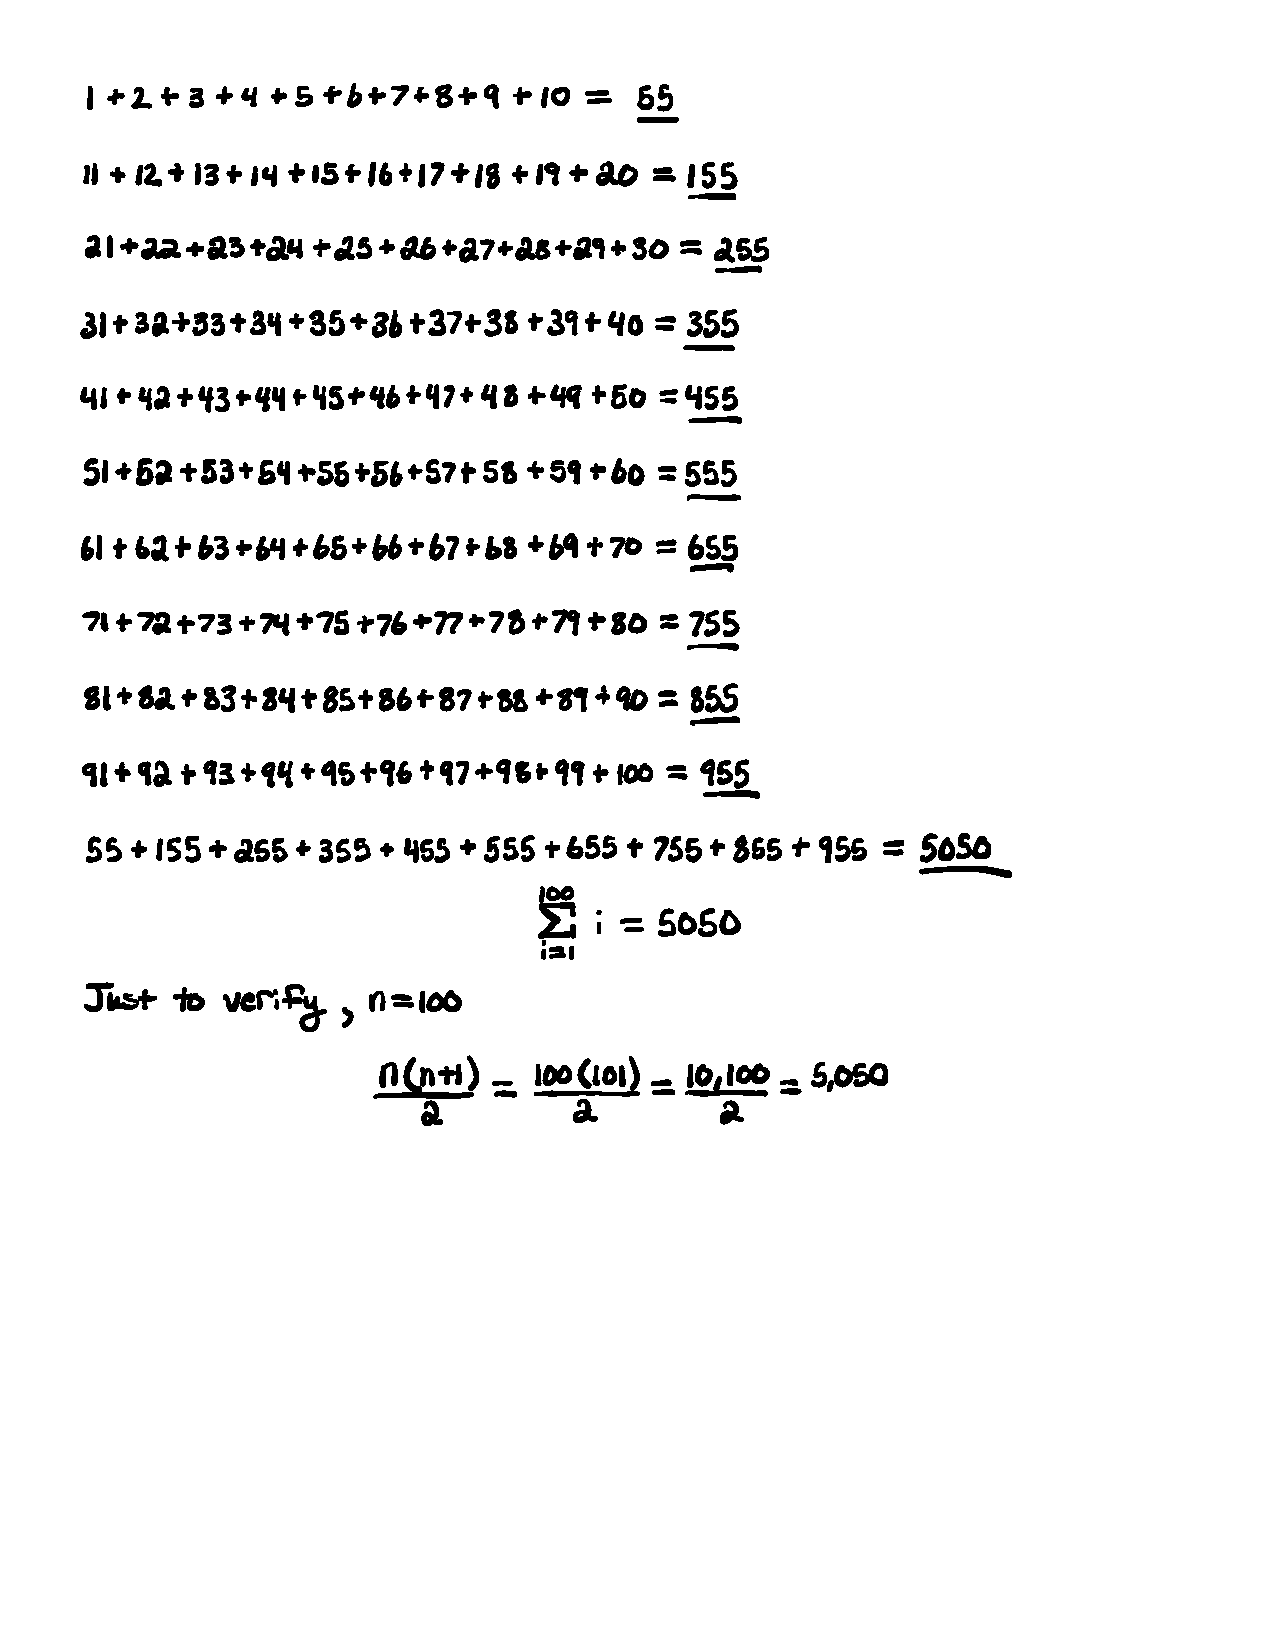
\includepdf[pages={-}, pagecommand={\thispagestyle{fancy}}, width=\paperwidth, offset=0 0]{./PDF/Problem 1.pdf}
\end{problem}

% Problem 1 Summary
\begin{summary}{Problem 1 Summary}
    \begin{statement}{Procedure}
        \begin{itemize}
            \item Create a sum for all ten increments of 100.
            \item Sum up all ten increments to get a final value.
            \item Compare the result with the formula
            \begin{equation*}
                \sum_{i = 1}^{n} = \frac{n(n + 1)}{2}.
            \end{equation*}
        \end{itemize}
    \end{statement}
    \begin{statement}{Key Concepts}
        \begin{itemize}
            \item This problem encapsulates the counting of numbers from 1 to a given integer.
            \item We can compare the result from our method by hand with
            \begin{equation*}
                \sum_{i = 1}^{n} = \frac{n(n + 1)}{2}.
            \end{equation*}
        \end{itemize}
    \end{statement}
    \begin{statement}{Variations}
        \begin{itemize}
            \item We could be given a different range of values to find the sum of.
            \begin{itemize}
                \item We could perform the sum either by hand our with the above formula.
            \end{itemize}
        \end{itemize}
    \end{statement}
\end{summary}

% Problem 2
\begin{problem}{Problem 2}
    \begin{statement}{Problem Statement}
        Understanding summation notation is essential in computer science. There will be an exam question about summation notation. Review/practice the exercises \#29, \#31, \#32 on page 169 in Rosen 
        as needed. You may do these in the Workbook but only select the graded portion below to submit. Check your answers using \href{https://www.mathsisfun.com/numbers/sigma-calculator.html}{Math Is Fun}. \vspace*{1em}

        Pick any ONE example from 29, 31, 32 and do the following on a single page.

        \begin{itemize}
            \item Write the summation example chosen in summation notation.
            \item Write out the terms and solution by hand.
            \item Write, in text, a short python function to calculate this sum without using built in functions for sums.
            \item Answer “How are summations and For Loops related?"
        \end{itemize}
    \end{statement}

    \begin{highlight}[Solution - \#29]
        For this problem, I am going to do problem 29 from Rosen on page 169. Particularly part (d) of 29.

        \begin{enumerate}[label = \arabic*., start = 29]
            \item What are the values of these sums?
            \begin{enumerate}[label = (\alph*), start = 4]
                % \item $\sum_{k = 1}^{5}(k + 1)$ \vspace*{1em}
                % \begin{align*}
                %     \sum_{k = 1}^{5} (k + 1) & = (1 + 1) + (2 + 1) + (3 + 1) + (4 + 1) + (5 + 1) \\
                %     & = 2 + 3 + 4 + 5 + 6 = 20.
                % \end{align*}
                % \item $\sum_{j = 0}^{4}(-2)^{j}$ \vspace*{1em}
                % \begin{align*}
                %     \sum_{j = 0}^{4}(-2)^{j} & = (-2)^{0} + (-2)^{1} + (-2)^{2} + (-2)^{3} + (-2)^{4} \\
                %     & = 1 + (-2) + 4 + (-8) + 16 = 11.
                % \end{align*}
                % \item $\sum_{i = 1}^{10} (3)$ \vspace*{1em}
                % \begin{equation}
                %     \sum_{i = 1}^{10} (3) = 3 + 3 + 3 + 3 + 3 + 3 + 3 + 3 + 3 + 3 = 30.
                % \end{equation}
                \item $\sum_{j = 0}^{8}(2^{j + 1} - 2^{j})$
                \scriptsize{
                    \begin{align*}
                        \sum_{j = 0}^{8}(2^{j + 1} - 2^{j}) & = (2^{1} - 2^{0}) + (2^{2} - 2^{1}) + (2^{3} - 2^{2}) + (2^{4} - 2^{3}) + (2^{5} - 2^{4}) + (2^{6} - 2^{5}) + (2^{7} - 2^{6}) + (2^{8} - 2^{7}) + (2^{9} - 2^{8}) \\
                        & = (1) + (2) + (4) + (8) + (16) + (32) + (64) + (128) + (256) = 511.
                    \end{align*}
                }
                \normalsize
            \end{enumerate}
        \end{enumerate}
        The code for this summation in Python can be seen below.

    \begin{lstlisting}[style=stackoverflow, language=python]
    # Part d
    def PartD(j0,jn):
        result = 0
        for i in range(j0,jn + 1):
            result += (2**(i + 1) - 2**i)
        return result
    \end{lstlisting}

    \begin{lstlisting}[style=stackoverflow]
    # Function call with print statement
    print(f"The result from part (d) of problem 29 is: {PartD(0,8)}")
    # Output
    The result from part (d) of problem 29 is: 511
    \end{lstlisting}

        Summations and for loops are related in that they are being executed over a range of integers. In a summation, we are performing some sort of mathematical operation for a given index in the 
        range and then summing those results over the entire range. For loops do something similar but they aren't constrained to performing mathematical operations inside of them. They can be used
        for a myriad of different operations with summing being one of them.
    \end{highlight}
\end{problem}

% Problem 2 Summary
\begin{summary}{Problem 2 Summary}
    \begin{statement}{Procedure}
        \begin{itemize}
            \item Perform the sum for the expression $\sum_{j = 0}^{8}(2^{j + 1} - 2^{j})$ by hand.
            \item Write code in Python for a generalized range of this sum.
            \item Display the result and generate of the summary the problem.
        \end{itemize}
    \end{statement}
    \begin{statement}{Key Concepts}
        \begin{itemize}
            \item This problem depicts the use of summation notation and how it is applied for a specific expression.
            \item We can generalize this sum by writing a code in Python that will perform the sum.
            \item Summations and for loops are related in that they both perform operations over a given range.
        \end{itemize}
    \end{statement}
    \begin{statement}{Variations}
        \begin{itemize}
            \item We could be given a different expression.
            \begin{itemize}
                \item In this case we would perform the same procedure for calculating the sum.
            \end{itemize}
        \end{itemize}
    \end{statement}
\end{summary}

% Problem 3
\begin{problem}{Problem 3}
    \begin{statement}{Problem Statement}
        Do \#3, \#9 and \#13 as needed page 168 for practice. Do \#12 b) and c) with explanation on this page.
    \end{statement}

    \begin{highlight}[Solution - \#12]
        \begin{enumerate}[label = \arabic*., start = 12]
            \item Show that the sequence $\{a_{n}\}$ is a solution of the recurrence relation $a_{n} = -3a_{n-1} + 4a_{n-2}$ if
        \end{enumerate}
        
        \begin{enumerate}[label = (\alph*), start = 2]
            \item $a_{n} = 1$
            \begin{align*}
                -3a_{n-1} + 4a_{n-2} & = -3(1) + 4(1) & \text{(Substitution)} \\
                & = -3 + 4 & \text{(Simplification)} \\
                & = 1 & \text{(Addition)} \\
                & = a_{n} & \text{(Substitution)}
            \end{align*}
            \item $a_{n} = (-4)^{n}$
            \begin{align*}
                -3a_{n-1} + 4a_{n-2} & = -3(-4)^{n - 1} + 4(-4)^{n - 2} & \text{(Substitution)} \\
                & = -3(-4)^{n}(-4)^{-1} + 4(-4)^{n}(-4)^{-2} & \text{(Algebra)} \\
                & = -3(-4)^{n}(-4)^{-1} + 4(-4)^{n}(-4)^{-1}(-4)^{-1} & \text{(Algebra)} \\
                & = (-4)^{n}(-3(-4)^{-1} + 4(-4)^{-1}(-4)^{-1}) & \text{(Factoring)} \\
                & = (-4)^{n}\Bigg(\frac{-3}{-4} + \frac{4}{(-4)\cdot(-4)}\Bigg) & \text{(Simplification)} \\
                & = (-4)^{n}\Bigg(\frac{3}{4} + \frac{4}{16}\Bigg) & \text{(Simplification)} \\
                & = (-4)^{n}\Bigg(\frac{3}{4} + \frac{1}{4}\Bigg) & \text{(Simplification)} \\
                & = (-4)^{n}(1) & \text{(Addition)} \\
                & = (-4)^{n} & \text{(Simplification)} \\
                & = a_{n} & \text{(Substitution)}
            \end{align*}
        \end{enumerate}

        When showing that a sequence is a solution to a recurrence relation we first need to substitute in the provided sequence into the recurrence relation. After this substitution we then need to
        carry out the algebra and show that the resulting algebra will result in the provided sequence.

        For part (b) of this problem, the sequence that was provided to us was a constant. In this case, the terms $a_{n-1}$ and $a_{n-2}$ have no effect on the constant term and we show that resulting
        algebra will be equal to the sequence that was provided to us. In part (c), when we insert $a_{n} = (-4)^{n}$ into the recurrence relation we have to apply the terms $a_{n-1}$ and $a_{n-2}$ to 
        the provided sequence. When we do this and carry out the algebra we get back the sequence that was provided to us. These relations always end with the LHS of the recurrence relation being equal
        to $a_{n}$.
    \end{highlight}
\end{problem}

% Problem 3 Summary
\begin{summary}{Problem 3 Summary}
    \begin{statement}{Procedure}
        \begin{itemize}
            \item Start with the recurrence relation and substitute the recurrence relation into it.
            \item Perform the necessary algebra to express the substituted sequence in its simplest form.
            \item Show that the simplest form is equal to the recurrence relation.
        \end{itemize}
    \end{statement}
    \begin{statement}{Key Concepts}
        \begin{itemize}
            \item When showing that a sequence is a solution for a recurrence relation, we first substitute the sequence into the recurrence relation.
            \item For sequences that are constants, it does not matter what the recurrence relation is, the sequences will be unchanged.
            \item The methodology for showing that a sequence is a solution to a recurrence relation is showing that once substituted, the algebra will simplify to the original recurrence relation.
        \end{itemize}
    \end{statement}
    \begin{statement}{Variations}
        \begin{itemize}
            \item We could be given a different recurrence relation and sequence.
            \begin{itemize}
                \item We would then perform the same procedure of substituting the sequence into the recurrence relation and then going through the necessary algebra that is needed to arrive at the
                original recurrence relation.
            \end{itemize}
        \end{itemize}
    \end{statement}
\end{summary}

% Problem 4
\begin{problem}{Problem 4}
    \begin{statement}{Problem Statement}
        For all positive integers $n, 1*2 + 2*3 + \dots + n(n + 1) = n(n + 1)(n + 2)/3$.
    \end{statement}

    \begin{highlight}[Solution]
        \noindent \textbf{Theorem:} For all positive integers, the sum of the products of $n$ consecutive integers is one third the product of $n(n + 1)(n + 2)$. Namely,
        \begin{equation*}
            \forall n \in \mathbb{Z}^{+}, \sum_{i = 1}^{n}(i(i + 1)) = \frac{n(n + 1)(n + 2)}{3}.
        \end{equation*}

        \noindent \textbf{Proof:} By mathematical induction. \vspace*{1em}

        \noindent \textbf{Base Case:} With $P(n) = \frac{n(n + 1)(n + 2)}{3}$, $P(1)$ is 

        \begin{equation*}
            P(1) = \frac{1(1 + 1)(1 + 2)}{3} = \frac{1(2)(3)}{3} = \frac{6}{3} = 2 = 1 \cdot 2.
        \end{equation*}

        \noindent \textbf{Inductive Hypothesis:} There is an arbitrary positive integer $k$ such that 

        \begin{equation*}
            1 \cdot 2 + 2 \cdot 3 + \dots + k(k + 1) = \frac{k(k + 1)(k + 2)}{3}.
        \end{equation*}

        \noindent \textbf{Inductive Step:} If 

        \begin{equation*}
            1 \cdot 2 + 2 \cdot 3 + \dots + k(k + 1) = \frac{k(k + 1)(k + 2)}{3}.
        \end{equation*}
        then 

        \begin{equation*}
            1 \cdot 2 + 2 \cdot 3 + \dots + k(k + 1) + (k + 1)(k + 2) = \frac{(k + 1)(k + 1 + 1)(k + 2 + 1)}{3} = \frac{(k + 1)(k + 2)(k + 3)}{3}.
        \end{equation*}

        \noindent \textbf{Induction Proof:}
        \horizontalline{0}{-1}
        \footnotesize{
            \begin{align*}
                1 \cdot 2 + 2 \cdot 3 + \dots + k(k + 1) + (k + 1)(k + 2) & = \frac{k(k + 1)(k + 2)}{3} + (k + 1)(k + 2) & \text{(Adding $(k + 1)(k + 2)$ To Each Side)} \\
                & = \frac{k(k + 1)(k + 2)}{3} + \frac{3(k + 1)(k + 2)}{3} & \text{(Algebra)} \\
                & = \frac{k(k + 1)(k + 2) + 3(k + 1)(k + 2)}{3} & \text{(Adding Fractions)} \\
                & = \frac{(k + 1)(k + 2)(k + 3)}{3} & \text{(Factoring $(k + 1)(k + 2)$)}
            \end{align*}
        }
        \horizontalline{-1}{0}
        \normalsize
        Consequently, we thus have $P(1)$ and $\forall k \in \mathbb{Z}^{+}, P(k) \rightarrow P(k + 1)$, so by the principle of mathematical induction, it follows that $P(n)$ is true for all positive
        integers $n$. \qed
    \end{highlight}
\end{problem}

% Problem 4 Summary
\begin{summary}{Problem 4 Summary}
    \begin{statement}{Procedure}
        \begin{itemize}
            \item Begin by stating the original theorem.
            \item State that the proof is going to be done with the method of mathematical induction.
            \item Calculate the base case of the theorem.
            \item State the inductive hypothesis (substitute $k$ for the other variable in the expression).
            \item State the inductive step (substitute $k + 1$ for every $k$ in the inductive hypothesis).
            \item Start with the induction hypothesis, transform it into the inductive step, and proceed to prove `then' part of the inductive step.
            \item Conclude the proof with showing that $P(\text{base case}) \rightarrow P(\text{inductive step})$.
        \end{itemize}
    \end{statement}
    \begin{statement}{Key Concepts}
        \begin{itemize}
            \item This problem showcases the method of a proof by induction.
        \end{itemize}
    \end{statement}
    \begin{statement}{Variations}
        \begin{itemize}
            \item We could be given a different theorem.
            \begin{itemize}
                \item Perform the same procedure as depicted in this problem making sure to use the correct base case for the new theorem.
            \end{itemize}
        \end{itemize}
    \end{statement}
\end{summary}

% Problem 5
\begin{problem}{Problem 5}
    \begin{statement}{Problem Statement}
        For all positive integers $n, 1^{3} + 2^{3} + 3^{3} + 4^{3} + \dots + n^{3} = (n(n + 1)/2)^{2}$.
    \end{statement}

    \begin{highlight}[Solution]
        \noindent \textbf{Theorem:} For all positive integers, the sum of the cube of integers is the square of one half of the product of $n(n + 1)$. Namely,

        \begin{equation*}
            \forall n \in \mathbb{Z}^{+}, \sum_{i = 1}^{n} (i^{3}) = \Big(\frac{n(n + 1)}{2}\Big)^{2}.
        \end{equation*}

        \noindent \textbf{Proof:} By mathematical induction. \vspace*{1em}

        \noindent \textbf{Base Case:} With $P(n) = \Big(\frac{n(n + 1)}{2}\Big)^{2}$, $P(1)$ is 

        \begin{equation*}
            P(1) = \Big(\frac{1(1 + 1)}{2}\Big)^{2} = \Big(\frac{(1)(2)}{2}\Big)^{2} = (1)^{2} = 1 = 1^{3}.
        \end{equation*}

        \noindent \textbf{Inductive Hypothesis:} There is an arbitrary positive integer $k$ such that

        \begin{equation*}
            1^{3} + 2^{3} + 3^{3} + 4^{3} + \dots + k^{3} = \Big(\frac{k(k + 1)}{2}\Big)^{2}.
        \end{equation*}

        \noindent \textbf{Inductive Step:} If 

        \begin{equation*}
            1^{3} + 2^{3} + 3^{3} + 4^{3} + \dots + k^{3} = \Big(\frac{k(k + 1)}{2}\Big)^{2}.
        \end{equation*}
        then

        \begin{equation*}
            1^{3} + 2^{3} + 3^{3} + 4^{3} + \dots + k^{3} + (k + 1)^{3} = \Big(\frac{(k + 1)(k + 1 + 1)}{2}\Big)^{2} = \Big(\frac{(k + 1)(k + 2)}{2}\Big)^{2}.
        \end{equation*}

        \noindent \textbf{Induction Proof:}
        \horizontalline{0}{-1}
        \footnotesize{
            \begin{align*}
                1^{3} + 2^{3} + 3^{3} + 4^{3} + \dots + k^{3} + (k + 1)^{3} & = \Big(\frac{k(k + 1)}{2}\Big)^{2} + (k + 1)^{3} & \text{(Adding $(k + 1)^{3}$ To Each Side)} \\
                & = \frac{k^{2}(k + 1)^{2}}{4} + (k + 1)^{3} & \text{(Carrying Out Square Of First Term)} \\
                & = \frac{k^{2}(k + 1)^{2}}{4} + \frac{4(k + 1)^{3}}{4} & \text{(Algebra)} \\
                & = \frac{k^{2}(k + 1)^{2} + 4(k + 1)^{3}}{4} & \text{(Adding Fractions)} \\
                & = \frac{(k + 1)^{2}(k^{2} + 4(k + 1))}{4} & \text{(Factoring $(k + 1)^{2}$)} \\
                & = \frac{(k + 1)^{2}(k^{2} + 4k + 4)}{4} & \text{(Distribution)} \\
                & = \frac{(k + 1)^{2}(k + 2)(k + 2)}{4} & \text{(Polynomial Factorization)} \\
                & = \frac{(k + 1)^{2}(k + 2)^{2}}{4} & \text{(Grouping Like Terms)} \\
                & = \Big(\frac{(k + 1)(k + 2)}{2}\Big)^{2} & \text{(Simplification)}
            \end{align*}
        }
        \normalsize
        \horizontalline{-1}{0}
        Consequently, we thus have $P(1)$ and $\forall k \in \mathbb{Z}^{+}, P(k) \rightarrow P(k + 1)$, so by the principle of mathematical induction, it follows that $P(n)$ is true for all positive
        integers $n$. \qed
    \end{highlight}
\end{problem}

% Problem 5 Summary
\begin{summary}{Problem 5 Summary}
    \begin{statement}{Procedure}
        \begin{itemize}
            \item Begin by stating the original theorem.
            \item State that the proof is going to be done with the method of mathematical induction.
            \item Calculate the base case of the theorem.
            \item State the inductive hypothesis (substitute $k$ for the other variable in the expression).
            \item State the inductive step (substitute $k + 1$ for every $k$ in the inductive hypothesis).
            \item Start with the induction hypothesis, transform it into the inductive step, and proceed to prove `then' part of the inductive step.
            \item Conclude the proof with showing that $P(\text{base case}) \rightarrow P(\text{inductive step})$.
        \end{itemize}
    \end{statement}
    \begin{statement}{Key Concepts}
        \begin{itemize}
            \item This problem showcases the method of a proof by induction.
        \end{itemize}
    \end{statement}
    \begin{statement}{Variations}
        \begin{itemize}
            \item We could be given a different theorem.
            \begin{itemize}
                \item Perform the same procedure as depicted in this problem making sure to use the correct base case for the new theorem.
            \end{itemize}
        \end{itemize}
    \end{statement}
\end{summary}

% Problem 6
\begin{problem}{Problem 6}
    \begin{statement}{Problem Statement}
        You may use PythonTutor or Runestone's code lens to help you understand. Do \#3 (Ungraded on your own). Then answer here \#4 from page 370, by hand, show work. Provide brief insight/explanation/notes 
        about how this is different and/or the same as your RSA code.
    \end{statement}

    \begin{highlight}[Solution - \#4]
        \begin{enumerate}[label = \arabic*., start = 4]
            \item Trace Algorithm 3 when it finds gcd(12, 17). That is, show all the steps used by Algorithm 3 to find gcd(12, 17). \vspace*{1em}
            
            \noindent \textbf{Algorithm 3:} \vspace*{1em}

            \textbf{procedure} gcd($a, b$: nonnegative integers with $a < b$) \newline
            if $a = 0$ then return $b$ \newline
            else return gcd($b \modulo a, a$) \newline
            \{output is gcd($a, b$)\} \newline

            \noindent \textbf{Trace Of Algorithm 3:} \vspace*{1em}

            We are aiming to calculate the gcd(12, 17). In each execution of this recursive algorithm we will denote the updated value for $a$ as $a'$ and $b$ as $b'$.
            \begin{align*}
                \text{Initial Iteration: } & \text{gcd($12,17$)} & a = 12, b = 17 \\
                & a \neq 0 \therefore \text{ gcd($17 \modulo 12 = 5, 12$)} & a' = 5, b' = 12 \\
                \text{Second Iteration: } & \text{gcd($5,12$)} & a = 5, b = 12 \\
                & a \neq 0 \therefore \text{ gcd($12 \modulo 5 = 2, 5$)} & a' = 2, b' = 5 \\
                \text{Third Iteration: } & \text{gcd($2,5$)} & a = 2, b = 5 \\
                & a \neq 0 \therefore \text{ gcd($5 \modulo 2 = 1$, 2)} & a' = 1, b' = 2 \\
                \text{Fourth Iteration: } & \text{gcd($1,2$)} & a = 1, b = 2 \\
                & a \neq 0 \therefore \text{ gcd($2 \modulo 1 = 0$, 1)} & a' = 0, b' = 1 \\
                \text{Fifth Iteration: } & \text{gcd($0,1$)} & a = 0, b = 1 \\
                & a = 0 \therefore \text{return $b$, $b = 1$} &
            \end{align*}

            Following the procedure of algorithm 3 we see that gcd(12,17) = 1.
        \end{enumerate}

        \noindent \textbf{Synopsis:} \vspace*{1em}

        Algorithm 3 is utilizing recursion to calculate the gcd of two integers. This algorithm is immediately different than that of the algorithm in our RSA project because it utilizes recursion.
        Our algorithm in RSA because it is utilizing a while loop inside the algorithm (at least in my case) until a certain condition is met for a value that is calculated inside the loop. The EEA
        algorithm in our project is also returning the Bezout coefficients for two integers and algorithm 3 is only returning the gcd of two integers.
    \end{highlight}
\end{problem}

% Problem 6 Summary
\begin{summary}{Problem 6 Summary}
    \begin{statement}{Procedure}
        \begin{itemize}
            \item Iterate through the recursive algorithm by performing the operation that is defined in the algorithm.
            \item Update the input parameters from the return values that are returned from one iteration until the break condition is reached.
            \item Show what the final return value of the algorithm will be after the break condition has been reached.
        \end{itemize}
    \end{statement}
    \begin{statement}{Key Concepts}
        \begin{itemize}
            \item This problem showcases the method of how a recursive algorithm is performed.
            \item Each iteration of a recursive algorithm will return values that are then fed into the algorithm again until the break condition is reached.
        \end{itemize}
    \end{statement}
    \begin{statement}{Variations}
        \begin{itemize}
            \item We could be given a different algorithm to analyze for what the algorithm will return.
            \begin{itemize}
                \item We would then iterate through each function call until the break condition has been reached.
            \end{itemize}
        \end{itemize}
    \end{statement}
\end{summary}

% Problem 7 
\begin{problem}{Problem 7}
    \begin{statement}{Problem Statement}
        Do \#5 (Ungraded on your own). Do and show \#6 page 370, by hand, show work. Provide brief insight/explanation/notes about how this is different and/or the same as your RSA code.
    \end{statement}

    \begin{highlight}[Solution - \#6]
        \begin{enumerate}[label = \arabic*., start = 6]
            \item Trace Algorithm 4 when it is given $m = 7, n = 10$, and $b = 2$ as input. That is, show all the steps Algorithm 4 uses to find $2^{10} \modulo 7$. \vspace*{1em}
            
            \noindent \textbf{Algorithm 4:} \vspace*{1em}

            \textbf{procedure} mpower($b, n, m$: integers with $b > 0$ and $m \geq 2, n \geq 0$) \newline
            if $n = 0$ then \newline
            \hspace*{10pt} return 1 \newline
            else if $n$ is even then \newline
            \hspace*{10pt} return mpower$(b,n/2,m)^{2} \modulo m$ \newline
            else \newline
            \hspace*{10pt} return (mpower$(b,\lfloor n/2 \rfloor,m)^{2} \modulo m \cdot b \modulo m$) $\modulo m$ \newline
            \{output is $b^{n} \modulo m$\} \newline

            We are aiming to calculate $b^{n} \modulo m$. In each execution of this recursive algorithm we will denote the updated value for $b$ as $b'$, $n$ as $n'$, and $m$ as $m'$.
            \footnotesize{
                \begin{align*}
                    \text{Initial Iteration: } & \text{mpower(2,10,7)} & b = 2, n = 10, m = 7 \\
                    & n \neq 0, n \text{ is even} \therefore \text{ return \text{mpower}}(2,5,7)^{2} \modulo 7 & b = 2, n' = 5, m = 7 \\
                    \text{Second Iteration: } & \text{mpower(2,5,7)} & b = 2, n = 5, m = 7 \\
                    & n \neq 0, n \text{ is odd} \therefore \text{ return }(\text{mpower}(2,2,7)^{2} \modulo 7 \cdot 2) \modulo 7 & b = 2, n' = 2, m = 7 \\
                    \text{Third Iteration: } & \text{mpower(2,2,7)} & b = 2, n = 2, m = 7 \\
                    & n \neq 0, n \text{ is even} \therefore \text{ return \text{mpower}}(2,1,7)^{2} \modulo 7 & b = 2, n' = 1, m = 7 \\
                    \text{Fourth Iteration: } & \text{mpower(2,1,7)} & b = 2, n = 1, m = 7 \\
                    & n \neq 0, n \text{ is odd} \therefore \text{ return }(\text{mpower}(2,0,7)^{2} \modulo 7 \cdot 2) \modulo 7 & b = 2, n' = 0, m = 7 \\
                    \text{Fifth Iteration: } & \text{mpower(2,0,7)} & b = 2, n = 0, m = 7 \\
                    & n = 0 \therefore \text{ return 1} &
                \end{align*}
            }
            \normalsize
            Now using the results from all of the recursive calls we have
            \footnotesize{
                \begin{align*}
                    \text{Fourth Iteration Result } & = (\text{mpower}(2,0,7)^{2} \cdot 2) \modulo 7 = (1^{2} \modulo 7 \cdot 2) \modulo 7 = (1 \cdot 2) \modulo 7 = 2 \modulo 7 = 2 \\
                    \therefore & \text{ mpower}(2,1,7) = 2 \\
                    \text{Third Iteration Result } & = (\text{mpower}(2,1,7)^{2}) \modulo 7 = 2^{2} \modulo 7 = 4 \modulo 7 = 4 \\
                    \therefore & \text{ mpower}(2,2,7) = 4 \\
                    \text{Second Iteration Result } & = (\text{mpower}(2,2,7)^{2} \cdot 2) \modulo 7 = (4^{2} \modulo 7 \cdot 2) \modulo 7 = (2 \cdot 2) \modulo 7 = 4 \modulo 7 = 4 \\
                    \therefore & \text{ mpower}(2,5,7) = 4 \\
                    \text{Initial Iteration Result } & = (\text{mpower}(2,5,7)^{2}) \modulo 7 = 4^{2} \modulo 7 = 16 \modulo 7 = 2 \\
                    \therefore & \text{ mpower}(2,10,7) = 2
                \end{align*}
            }
            \normalsize
            Climbing back up the recursive tree we can see that $2^{10} \modulo 7 = 2$.            
        \end{enumerate}
        
        \textbf{Synopsis:} \vspace*{1em}

        This algorithm that we used in this problem is different from our FME algorithm in the RSA project as this algorithm is using recursion to calculate the FME of integers. In our RSA project
        we used a for loop that iterated over the digits in a binary number and performed a specific operation with that digit depending on its value. In my opinion, this algorithm is a lot more
        difficult to interpret because of the recursive calls. The fact that this recursive algorithm in particular returns a value with the function call again makes it more difficult to interpret.
    \end{highlight}
\end{problem}

% Problem 7 Summary
\begin{summary}{Problem 7 Summary}
    \begin{statement}{Procedure}
        \begin{itemize}
            \item Iterate through the recursive algorithm by performing the operation that is defined in the algorithm.
            \item Update the input parameters from the return values that are returned from one iteration until the break condition is reached.
            \item Climb back up the recursive tree to show what each branch of the tree will evaluate to.
            \item Show what the final branch of the tree will evaluate to at the end of the recursive calls.
        \end{itemize}
    \end{statement}
    \begin{statement}{Key Concepts}
        \begin{itemize}
            \item This problem showcases the method of how a recursive algorithm is performed.
            \item Each iteration of a recursive algorithm will return values that are then fed into the algorithm again until the break condition is reached.
            \item We can use results from branches that are farther from the root of the tree to incur what the initial call of the algorithm will be.
        \end{itemize}
    \end{statement}
    \begin{statement}{Variations}
        \begin{itemize}
            \item We could be given a different algorithm to analyze for what the algorithm will return.
            \begin{itemize}
                \item We would then iterate through each function call until the break condition has been reached.
                \item We then would use results from the last call to incur what the previous calls evaluate to.
            \end{itemize}
        \end{itemize}
    \end{statement}
\end{summary}